\section{Eliminación de duplicados}\label{sec:eliminacion-duplicados}

La eliminación de estudios duplicados se llevó a cabo mediante la herramienta de gestión bibliográfica Mendeley. Tras la recopilación inicial, todos los registros fueron importados a dicha plataforma, la cual permitió la identificación y eliminación automática de publicaciones redundantes. Este proceso resultó en la exclusión de \textbf{tres} artículos duplicados, reduciendo el total de estudios a 156. La \autoref{fig:eliminacion-duplicados} presenta una representación gráfica de estos resultados.

\begin{figure}[H]
	\centering
	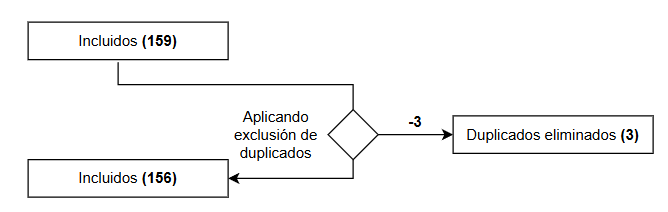
\includegraphics[width=0.9\textwidth]{mainmatter/II-desarrollo-metodologico/sms/imagenes/eliminacion-duplicados.png}
	\caption{Diagrama del proceso de eliminación de resultados duplicados}
	\label{fig:eliminacion-duplicados}
\end{figure}
